\documentclass{include/protokollclass}

\usepackage{pdfpages}
\usepackage{booktabs}
\usepackage{tcolorbox}
\usepackage[ngerman]{babel}

%% ---------------------------------
%% |    Commands for neat stuff    |
%% ---------------------------------

\newcommand{\gqm}[1]{\glqq#1\grqq}
\newcommand{\red}[1]{\textcolor{red}{#1}}
\newcommand{\green}[1]{\textcolor{green}{#1}}
\newcommand{\purple}[1]{\textcolor{purple}{#1}}
\newcommand{\blue}[1]{\textcolor{blue}{#1}}

\title{Der Schwarze Tod}
\author{DerHauge\thanks{Rahmenhandlung}, Quizznor\thanks{Typesetting}}

%% --------------------
%% |    Main Story    |
%% --------------------

\begin{document}

\maketitle
\tableofcontents

\chapter{Informationen}
%!TEX root = ../main.tex

\section{Allgemeines}

%!TEX root = ../main.tex

\textbf{Wo?}            -  mittelalterliches Hamburg \\
\textbf{Wann?}          -  1350 n. Chr. \\
\textbf{Spielerzahl?}   -  3 - 5 \\
\textbf{Schwierigkeit?} -  einfach - mittel \\
\textbf{Spieldauer?}    -  3-4 Stunden

\section{Anmerkungen für Spielleiter}

Die Formatierung ist nicht zufällig gewählt. Im Verlauf des Abenteuers werden spezielle Informationen wie folgt verdeutlicht:

\begin{itemize}
  \item \textit{Kursive Texte}
  Alles, was \textit{kursiv} geschrieben ist, kann wörtlich vorgetragen werden. Dabei handelt es sich meistens um die Einleitungen der einzelnen Abschnitten oder um wörtliche Rede in Gesprächen.

  \item \textbf{Raumbeschreibungen/Ortsbeschreibungen}
  Diese Beschreibungen verweisen auf die Einrichtung eines Raums oder die Beschaffenheit eines Ortes und sind \textbf{fett} gedruckt. Raumbeschreibungen beschreiben meistens alles, was innerhalb eines Gebäudes zu sehen ist, Ortsbeschreibungen hingegen beschreiben, was draußen ist.

  \item \red{\textbf{Szenen und Interaktionen}}
  Die Abschnitte sind in Szenen und Interaktionen unterteilt. Damit es einfacher ist, dorthin zu navigieren, sind diese \red{rot} markiert. Szenen geben eine Handlung vor, die sich den Spielern offenbart, wenn sie sich in einem Abschnitt befinden. Interaktionen ermöglichen optionale Handlungsstränge, die den Spielern entgehen können, wenn sie nicht die entsprechenden Aktionen durchführen oder sich für die entsprechende Option entscheiden.

  \item \green{\textbf{Moral}}
  Alle Stellen, an denen die Spieler mit moralischen Fragen konfrontiert werden, sind \green{grün} gekennzeichnet. Diese markieren Entscheidungen, die sich auf den Ausgang der Geschichte auswirken können.

  \item \purple{\textbf{Pestilenz}}
  Alle Stellen, an denen die Spieler in Kontakt mit der Pest kommen und gegebenenfalls Pestilenz anhäufen können, sind \purple{lila} markiert.
\end{itemize}


\section{Setting}

%!TEX root = ../main.tex

Wir schreiben das Jahr 1350. Hamburg wächst dank des erstarkenden Seehandels stetig und die Hanse trägt ihren Teil dazu bei. Täglich gehen am Rheinhafen Schiffe aus aller Herren Länder vor Anker, während vom Rathaus an der Troßtbrücke der Rat die Geschicke der Stadt lenkt. Es ist eine Zeit des Aufbruchs, aber auch eine Zeit der Angst. Denn neben Piraten und anderen finsteren Gestalten, die zunehmend in den Gassen der Stadt umherstreifen, greift etwas noch viel gefährlicheres um sich. Die Leute hatten bereits von einem „Schwarzen Tod" gehört, der binnen weniger Tage einen gesunden Mann seiner Lebenskraft zu berauben vermag. Nun scheint es so, als sei die Plage auch in die Wohnungen von Hamburg eingedrungen. Der düstere Geruch des Todes zieht durch die Docks und Armenviertel, während der Rat darüber entscheidet, was zu tun ist.

Und was auch immer das sein mag, es muss schnell geschehen.


\chapter{Charaktere}

%!TEX root = ../main.tex

\subsection{Ortsgebundene Charaktere}

Unter jedem Charakter ist eine Auflistung an Orten/Situationen zu finden, an denen der jeweilige Charakter in Erscheinung treten kann. Zur einfachen Navigation lassen sich diese Anklicken, sodass schnell und bequem zwischen Abenteuer und Informationen hin und her gewechselt werden kann.

\subsubsection*{Hanno - Der Totensammler}
\label{Hanno}

Hanno ist ein kleiner buckliger, zynischer aber freundlicher alter Mann. Zumindest sollte man vermuten, dass er alt ist. So richtig sicher kann man das nicht sagen. Seine Kleidung besteht größtenteils aus Flicken. Er hat eine kratzige Stimme und ist der Gruppe gegenüber grundlegend wohlgesonnen eingestellt, weiß aber auch, seine Informationen zu Geld zu machen. Er taucht eventuell im Sitz des Beirates auf.

Kapitel 2 - Im Sitz des Beirats (gehe zu \blue{\ref{tot}})

\subsubsection*{Frieder - Der Kutscher}
\label{Frieder}

Ein ängstlicher, nicht gerade heller Typ, der die Gruppe nach Eeksdurf fährt. Er ist zartbesaitet. Er kann den Spielern nichts weiter erzählen.

\subsubsection*{General zu Brügge - Der Kürzermacher}
\label{Brügge}

Ein um die 50 Jahre alter, dickbäuchiger und hochdekorierter Mann mit grauem und gut gepflegtem Bart. Der General nimmt alles sehr genau, nicht nur den perfekten Sitz seiner Uniform. Er mag hitzig sein, ist aber keineswegs dumm. Seine Karriere begann in der Schlacht um die Handelsrouten Hamburgs mit den Piraten der Region. Er konnte trotz der neuen Verträge den Frieden nie akzeptieren.

\red{\textbf{Probe auf Gesellschaft}: Sein Beiname lautet „Der Kürzermacher“ und wurde ihm gegeben, weil Piraten in seiner Gefangenschaft fast ausschließlich den Tod durch Enthauptung finden}

\textbf{Auftreten}:

Kapitel 2 - Im Sitz des Beirats (gehe zu \blue{\ref{militär}})

\subsubsection*{Mutter und Kind}
\label{MutterKind}

Das Kind kommt ganz offensichtlich aus dem Armenviertel. Es klammert sich an die Hand seiner Mutter, die bereits schwer von der Pest gezeichnet ist. Es ist spindeldürr, ausgehungert und die Lumpen hängen an seinem Körper herunter. Es ist schmutzig und schüchtern. Die Mutter ist dick in mehrere Laken Kleidung eingehüllt. Sie möchte ihr Kleines retten, so lange es noch geht. Die Gruppe kann nicht viel von ihrem Gesicht erkennen, doch die knochige Hand, die die Hand des Kindes hält, lässt nichts Gutes erahnen. Sie ist tiefgläubig und vertraut auf das Gerücht, dass in der Kirche St. Petri Rettung zu finden ist.

\textbf{Auftreten}:

Kapitel 2 - Im Sitz des Beirats (gehe zu \blue{\ref{kind}})

\subsubsection*{Didrich von Sinnfeld - Der Pestdoktor}
\label{Didrich}

Er strahlt eine unangenehme Aura aus. Seine dünne Nase ist spitz zulaufend, so spitz wie ein Vogelschnabel. Wache, umtriebige Augen schauen aus tiefen Höhlen. Er ist spindeldürr und trägt sein braunes Haar kraus in Locken auf dem Kopf. Er ist gebildet und nimmt nichts für gegeben, er überprüft Theorien lieber selbst. Er wirkt herablassend und gekünstelt, weil er sich seiner Intelligenz bewusst ist. Bei seiner Forschung wandelt er nicht nur auf dem Grat zur Morallosigkeit, er überschreitet diesen schmalen Grat auch bewusst, wo es seiner Meinung nach nötig ist. Sein Stand und Vermögen ermöglichen ihm einen Lebensstil, in dem er sich mit Rätseln der Natur und den Belangen der Welt auseinandersetzen kann. Auf seinen Reisen, aber auch durch sein Geschäft, lernt er oft allerlei Neues kennen, das man so in Hamburg noch nicht kennt. Seine Familie ist hoch angesehen und bewegt sich in Adelskreisen.

\red{\textbf{Info}: Didrich erforscht heimlich die Pest und ist der Mann in Mantel und Vogelmaske.}

\textbf{Auftreten}:

Kapitel 2 - Im Sitz des Beirats (gehe zu \blue{\ref{kind}})


\subsection{Hafen}

Der Hafen steht seit Hamburgs Beitritt zur Hanse vor etwa 30 Jahren im Mittelpunkt der städtischen Wirtschaft. Hier wächst der neue Wohlstand heran. Unzählige Waren und Handelsgüter werden Tag ein Tag aus umgeschlagen, und mit ihnen kommen immer mehr Fremde in die Stadt. Eine ganz eigene Welt entsteht. Mit eigenen Regeln, die man erst lernen muss ...

\subsubsection*{Matrosen}
\label{Matrosen}

Es ist nicht verwunderlich, dass sich in der großen Hansestadt Matrosen tummeln. Manche sind gerade erst wieder nach langer Zeit an Land gekommen, andere werden demnächst wieder die Segel setzen. Die meisten sind am Hafen oft in einer der zahlreichen Kaschemmen zu finden, in denen alles bis auf Wasser ausgeschenkt wird.

\textbf{Auftreten}:

Kapitel 3 - Am Hafen (gehe zu \blue{\ref{Hafen}})

\subsubsection*{Hafenarbeiter}
\label{Hafenarbeiter}

Die Hafenarbeiter sind Teil des Wohlstandes der Hanse, auch wenn sie selbst an diesem Wohlstand nur in den wenigsten Fällen beteiligt sind. Ihre Aufgabe ist es, die Ladung der Schiffe zu löschen und Stoffe, Gewürze und Materialien in ihre angestammten Lagerhäuser zu bringen, von wo aus sie ihren Weg in die Hände der Reichen finden.

\red{\textbf{Info}: Fragt man sie danach, dann können sie den Charakteren genau sagen, wo welches Lagerhaus zu finden ist.}

\textbf{Auftreten}:

Kapitel 3 - Am Hafen (gehe zu \blue{\ref{Hafen}})

\subsubsection*{Prostituierte}
\label{Prostituierte}

Wo Matrosen sind, sind Prostituierte nicht weit. Für viele Frauen ist es der einzige Weg über die Runden zu kommen, doch sind sie auch Hüterinnen großer Geheimnisse. Schon so manchem Mann hat die körperliche Nähe die Zunge gelockert, sodass er nebst seinem Geld auch mehr oder weniger nützliche Informationen dagelassen hat. Die Prostituierten verstehen es, dieses Wissen zu Geld zu machen

\red{\textbf{Info}: Die Geschehnisse der Nacht kennen sie gut, können also auch berichten, dass in dem Lagerhaus eines gewissen Herrn von Sinnfeld einige Arbeiter verschwunden sind.}

\textbf{Auftreten}:

Kapitel 3 - Am Hafen (gehe zu \blue{\ref{Hafen}})

\subsubsection*{Aufseher der Hanse}
\label{Aufseher}

Die Aufseher haben ein scharfes Auge auf ihre Hafenarbeiter, denn auf wen würde es denn zurückfallen, wenn etwas Chili oder Zimt verloren gehen würde? Sie regieren die Hanse mit harter Hand und wenn jemand weiß, was wo zu sein hat, dann sie.

\red{\textbf{Info}: Gegen eine kleine Bestechung erzählen sie, dass eines der Lagerhäuser einem Herrn von Sinnfeld gehört.}

\textbf{Auftreten}:

Kapitel 3 - Am Hafen (gehe zu \blue{\ref{Hafen}})

\subsubsection*{Gert - Wirt des \gqm{Gelockten Hund}}
\label{Gert}

Ein kräftiger Mann, der keine Scherereien in seiner Schenke duldet, außer er verursacht sie selbst. Meist hält er sich im Hintergrund und gibt eine Suppe aus, deren Zutaten niemand kennt – oder kennen will. Gert ist schweigsam und redet nur, wenn er etwas Wichtiges zu sagen hat. Seine Stammgäste scheinen eine Ehrfurcht vor ihm zu haben, die sich der sporadische Besucher nicht recht erklären kann; vielleicht liegt es daran, dass Gert den „Gelockten Hund“ führt wie ein Kapitän sein Schiff.

Kapitel 3 - Am Hafen (gehe zu \blue{\ref{imhund}})

\subsubsection*{Gorich - Der Dithmarscher}
\label{Gorich}

Gorich der Dithmarscher unterscheidet sich äußerlich nicht von Gert dem Wirt, auch charakterlich sind die beiden nicht allzu verschieden. Gorich weiß sehr genau, wann er sich bedeckt halten muss und wann er zur Tat schreiten kann, ohne Gefahr zu laufen gefangen genommen zu werden. Gesucht und gefürchtet von der Hamburger Hanse, ist Gorich gerissen genug, um noch im Untergrund seinen Profit herauszuschlagen. Dennoch ist Profit nicht sein einziger Antrieb. Man mag es glauben oder nicht, aber seine Familie liegt ihm am Herzen, und für seine Kinder würde Gorich fast alles tun.

\textbf{Auftreten}:

Kapitel 2 - Im Sitz des Beirats (gehe zu \blue{\ref{militär}})
Kapitel 3 - Am Hafen (gehe zu \blue{\ref{imhund}})

\subsection{Kirche St. Petri}

Die Kirche zu Sankt Petri steht ganz im Zeichen des neuen Hamburger Wohlstands. Noch immer wird gebaut, aber man sieht ihr schon jetzt an, dass sie eines der zukünftigen Wahrzeichen der Handelsmetropole sein wird. Viele Menschen pilgern angesichts ihrer Machtlosigkeit gegenüber der Pest hierher, um Schutz und Trost zu suchen. Kranke und Verzweifelte säumen die Gänge, und der Geruch von Tod liegt in der Luft.


\subsubsection*{Pater Salus}
\label{Salus}

Pater Salus hat einen guten Ruf in seiner Gemeinde. Der etwas füllige Pfaffe ist bisher von der Krankheit verschont geblieben. Sein Kreuz, das er immer um den Hals trägt, ist so reich gestaltet wie die ganze Prunkkirche, in der er tätig ist. Salus ist ein gelehrter Mann, der den Dingen auf den Grund geht. So zieht er sogleich los, als er den Brief aus dem Hammerbrook erhält, um den Armen Lebensmittel zu bringen und ihnen zu helfen. Er hat herausgefunden, dass Menschen länger gesund bleiben, wenn sie nicht mit Kranken in Kontakt kommen. Wer von der Krankheit gezeichnet ist und andere anzustecken droht, wird deshalb in einem der hinteren Zimmer der Kirche „vorläufig“ gefangengenommen.

\subsubsection*{Gundel}
\label{Gundel}

Gundel kocht für die Männer am Nikolaifleet und ist dort sehr beliebt. Die Männer erzählen ihr alles, was in der Stadt vorgeht. Trotz ihres jungen Alters wird sie respektiert. Sie steht mit beiden Füßen fest auf dem Boden und weiß, was sie wert ist. Ihre Haare trägt Gundel zu einem dicken Zopf geflochten streng am Kopf, darüber ein Tuch, das zum einen die Haare im zaum hält, zum anderen den Schweiß von der Hitze in der Küche daran hindert ihr in die Augen zu fließen. Gundel ist nicht schlank - welche Köchin ist das schon? -, sondern hat eher eine Mutti-Statur. Über einem einfachen Kleid trägt sie eine fleckige Schürze. In ihrem Kleid verbirgt sie in eingenähten Taschen aber allerlei Nützliches, das sie bei Bedarf hervorzaubern kann. Sie ist generell sehr hilfsbereit und willigt daher ein, Didrich von Sinnfeld bei der Suche nach den Ursachen der Pest zu unterstützen.

\subsubsection*{Leichenfledderer}
\label{Leichenfledderer}

Wo es was zu holen gibt, sind auch die, die es holen. Die Gruppe entdeckt an den Leichenbergen wühlend ein Kind. Der Kleine stellt sich als Tom vor und sucht zwischen den toten Körpern nach Kostbarkeiten und Habseligkeiten, die er verkaufen kann, um sich durchzuschlagen. Seine Mutter ist bereits gestorben, einen Vater habe er nie gekannt, sagt er. Der Blondschopf ist klein und abgemagert, ein Straßenkind, eine verlorene Seele von der es in Hamburg immer mehr zu geben scheint.

\subsubsection*{Prediger}
\label{Prediger}

In der Mitte des Hauptraumes der Kirche entdecken die Spieler einen Prediger, der sich besonders auffällig benimmt. Er predigt für die Schutzsuchenden mit ausgeprägter Theatralität und gibt sich imposant. Sein Blick ist voller Sorge und Reue, aber auch mahnend. Doch die Gruppe sieht, dass er ein falscher Hund ist. Denn was er sagt, ist leicht zusammengefasst: Wer krank ist, hat gesündigt und erhält die verdiente Strafe. Gegen ein kleines weltliches Gut könne man sich bei ihm aber von einigen Sünden freikaufen.

\subsubsection*{Fleischer}
\label{Fleischer}

In der Nähe der Leichenberge steht eine übergewichtige, beeindruckende Gestalt. Fettige Schürze und riesige Hände, die fast schon an Pranken erinnern. Die öligen schwarzen Haare sind zu einem langen Pferdeschwanz zusammengebunden. Es ist der Fleischer der Gegend, der hier seine Waren anbietet. Dass ein Haufen toter Körper eine denkbar ungünstige Umgebung für sein Geschäft ist, leuchtet ihm nicht ein. Fleisch sei immerhin auch nichts anderes.

\subsubsection*{Allgemeine Beschreibung der Leute}
\label{Leute}

Die Kirche ist voller Menschen, die hier Schutz suchen. Sie lehnen an den Wänden des Hauptraumes, schütteln sich, liegen sich vor Schmerzen krümmend auf dem Boden. So viel Leid an einem Platz. Um den Prediger hat sich eine Traube gebildet, Hände greifen flehend nach den Ablassbriefen, die Betroffenen geben ihr letztes Hab und Gut für einen Funken Hoffnung.


\subsection{Eeksdurf}

Eeksdurf liegt vor den westlichen Toren der Stadt, am Rande des Eekshult. Die Bewohner des Ortes gehen den üblichen Handwerksberufen und der Landwirtschaft nach. Ein beschaulicher Ort. Binnen zweier Wochen starben oder erkrankten bereits über die Hälfte der Bewohner des Dörfchens. Das kann kein Zufall sein, vermuten einige im Dorf. Jemand sei mit dem Teufel im Bunde, wird gemutmaßt. Eine Hexenjagd entbrennt, vor der niemand sicher zu sein scheint.

\subsubsection*{Wolfgang - Bauer}
\label{Wolfgang}

Wolfgang ist der Rädelsführer des Mobs, der versucht, Ottildes Haus zu stürmen und Ruth zu finden. Er ist der Vater von Hermann, hat ein rüstiges Alter, zerrissene dreckige Kleider und eine Knubbelnase. Er ist etwa 1,50 Meter groß, hat rabenschwarze Haare und einen Rosenkranz, der als einziges Utensil sorgsam gehalten wird. Er sieht aus wie jemand, der harter körperlicher Arbeit nachgeht. Er ist sichtlich verunsichert aufgrund der vielen Toten und Kranken im Dorf und verlangt eine Erklärung. Er ist bereits mit der Pest in Berührung gekommen.

\textbf{Auftreten}:

Kapitel 4 - Der Weg nach Eeksdurf (gehe zu \blue{\ref{nachxd}})
Kapitel 4 - Der Mob (gehe zu \blue{\ref{mob}})
Kapitel 4 - Das Feuer (gehe zu \blue{\ref{feuer}})

\subsubsection*{Hermann - Bauer}
\label{Hermann}

Hermann ist Anfang 20 und hat langes blondes Haar, das auf seine Schultern fällt. Er hat Dreck im Gesicht, drei bis vier ausgefallene Zähne, ist kräftig gebaut, hat große schwielige Hände und ein Schönheitsmakel links über der Lippe. Hermann ist stockdumm. Er ist Wolfgangs Sohn und läuft diesem treudoof hinterher. Man sieht ihm an, dass er bereits mit der Pest in Berührung gekommen ist.

\textbf{Auftreten}:

Kapitel 4 - Das Feuer (gehe zu \blue{\ref{feuer}})

\subsubsection*{Kunibert - Bauer}
\label{Kunibert}

Kunibert hat kurze stoppelige blonde Haare, ist kräftig gebaut, verwitwet und war früher Minnesänger. Er ist ein typischer Mitläufer.

\subsubsection*{Otto - Bauer}
\label{Otto}

Bei genauerem Hinsehen entdecken die Spieler versteckte Pestbeulen an seinem Körper. Otto ist kräftig gebaut, hat einen starken Unterbiss und taumelt etwas beim Gehen.

\subsubsection*{Friedrich - Wirt}
\label{Friedrich}

Friedrich ist groß und hat lockiges schwarzes Haar. Die Zunge wurde ihm beim Versuch ihn und die Pest zu vertreiben herausgeschnitten, weswegen er stumm ist. Er ist gläubiger Jude.

\subsubsection*{Hildegart - Wirtin}
\label{Hildegart}

Hildegart ist eine kleine, zierliche Frau. Sie ist sehr bodenständig. Sie trägt ihr Haar kurzgeschnitten und ist gläubige Jüdin.

\subsubsection*{Ottilde - Kräuterfrau}
\label{Ottilde}

Die Kräuterfrau hat schlecht abrasierte Haare, einzelne Büschel sehen wie an der Kopfhaut angeklebt aus. Ottilde ist sehr klein im Vergleich zu den Spielern, sie misst nur zirka 1,30 Meter. Sie ist abgemagert und verängstigt gegenüber anderen Menschen. Sie hat Angst um ihre Tochter.

\textbf{Auftreten}:

Kapitel 4 - Eeksdurf (gehe zu \blue{\ref{inxd}})

\subsubsection*{Ruth}
\label{Ruth}

Ruth ist die Tochter der Kräuterfrau Ottilde. Sie ist freundlich, etwas naiv und hübsch. Sie hat rote Haare, weshalb es dem Dorf leicht fällt, sie zum Sündenbock zu erheben. Weil sie des öfteren dabei beobachtet wurde, wie sie Tote aus dem Dorf in die Scheune geschleppt hat, wird sie verdächtigt, mit dem Teufel im Bunde zu sein und Unheil über den Ort gebracht zu haben. Ruth ist verzweifelt und verängstigt. Sie hat sich auf einen Deal mit Didrich eingelassen und bald bemerkt, dass plötzlich viele Menschen im Dorf erkrankten. Ihr ist bewusst, dass das mit den Toten zusammenhängen muss, weshalb sie sich Vorwürfe macht.

\textbf{Auftreten}:

Kapitel 4 - Eeksdurf (gehe zu \blue{\ref{inxd}})

\subsection{Am Nikolaifleet}

Erst seit wenigen Jahren wächst am Nikolaifleet ein gewaltiges Lagerzentrum für die Waren aus aller Welt. Der neue Reichtum trägt hier Früchte, und in direkter Nähe zu Tee, Gewürzen und Tulpen siedeln sich die betuchteren Bürger Hamburgs in prächtigen Villen an. Alles scheint makellos und vom Chaos der übrigen Stadt unberührt. Fast schon zu makellos.

\subsubsection*{Der Mann in der Grube}
\label{Grubenmann}

Im Lagerhaus am Nikolaifleet findet die Gruppe einen gefesselten, schwerkranken Mann. Er ist ausgemergelt und sein Körper ist von Rattenbissen übersäht. Seine Haare hängen in Strähnen von seinem Kopf, die Wangenknochen treten deutlich hervor. Seine Kleidung ist zerschunden, war aber offenbar nie in einem wirklich ansehnlichen Zustand. Er ist schwach, dem Tode nah.

\subsubsection*{Hagen vom Fleet}
\label{Hagen}

Hagen ist ein groß gewachsener, blonder Mann Mitte 30. Er ist nicht verheiratet und hat keine Kinder. Er ist zwar etwas einfältig, aber keineswegs strohdoof. Außerdem ist er sehr geschäftstüchtig und nimmt keine Rücksicht auf Verluste. Er arbeitet am Nikolaifleet, wo er Waren stiehlt und diese an Dritte verkauft.

\subsubsection*{Beamtin des Handelsregisters}
\label{Beamtin}

Im Handelsregister erwartet die Gruppe eine typische Beamtin. Sie ist fein zurechtgemacht und kann die Regeln und Gesetze der Handelsaktivitäten im Schlaf herunterbeten. Was sie auf den Tod nicht ausstehen kann, ist wenn Unbefugte in ihr Büro hereinmarschieren und dumme Fragen stellen. Oder kluge Fragen. Oder Fragen generell. Als Frau in gehobener Position ist ihr bewusst, dass sie zu den Seltenheiten in Hamburg gehört. Sie hat sich ihren Stand hart erarbeitet und lässt sich von keinem Mann etwas sagen. Auf Frauen niederen Standes schaut sie herab.

\subsubsection*{Mitarbeiter des Handelsregisters}
\label{Mitarbeiter}

Die anderen Mitarbeiter des Handelsregisters sind zumindest Bekanntheiten der Stadt gegenüber offener eingestellt und helfen freundlich weiter, wenn sie angesprochen werden, auch wenn die geforderte Hilfe nicht ganz legal sein sollte.

\subsubsection*{Traudel - die Magd}
\label{Traudel}

Traudel ist die Magd von Didrich von Sinnfeld. Sie ist aufgeweckt und freundlich und beobachtet mit offenen Augen, was um sie herum vor sich geht. Sie ist eine gut geschulte Magd und keineswegs naiv. Sie weiß, dass sie es mit ihrer Anstellung wirklich gut getroffen hat, die Familie von Sinnfeld ist reich und behandelt ihre Bediensteten wirklich gut. Umso wichtiger ist es ihr, ihre Aufgaben zur vollsten Zufriedenheit zu erfüllen und ihren Dienstherren keiner Gefahr auszusetzen. Doch trotzdem ist und bleibt sie eine Magd, ein Kleingeist, wie ihr Dienstherr zu sagen pflegt. Was er in seinen Räumen so treibt, erschreckt sie ab und an und ist ihr auch immer mal nicht ganz geheuer.

\subsubsection*{Bettler}
\label{Bettler}

Wo es reiches Volk gibt, gibt es Bettler. Sie wissen genau, wo welche Familie wohnt und wer die Angestellten sind, die auch mal einen Rest aus der Küche herausrücken.

\subsubsection*{Pestdoktoren}
\label{Pestdoktoren}

Die Pest jagt nicht nur Schrecken ein, sie lockt auch viele selbsternannte Mediziner, die die Gelegenheit nutzen, ihre Experimente an den armen Opfern auszuprobieren. Die Gruppe entdeckt sogenannte Heiler, die auf offener Straße Aderlasse durchführen und den Kranken und Angehörigen Kräuterbündel, dubiose Tränke und Schutzmedaillons andrehen.

\subsubsection*{Händler}
\label{Händler}

Medaillons, Kräutermischungen, Schutzkleidung, Segenszettelchen – auf Hamburgs Straßen wird zur Zeit alles verkauft, was irgendwie gegen die Krankheit schützen könnte. Die Betonung liegt auf könnte, denn was die Krankheit auslöst, weiß keiner. Aber das ist kein Grund, nicht ein Geschäft aus der Angst der Bürger zu machen.

\subsubsection*{Hehler}
\label{Hehler}

Viele Tote hinterlassen viel Krempel, der verkauft werden kann. Die Hehler der Stadt wittern gute Geschäfte und verkaufen alles, was sich finden lässt – über ihre sonstigen Hehlerwaren hinaus.


\subsection{Hammerbrook – Die Armenviertel}

Wer im Armenviertel landet, freut sich über das Kleinste und erwartet das Schlimmste. Hier spürt man nichts vom neuen Reichtum. Dicht gedrängt leben hier Hafenarbeiter, einfache Leute und anderes Gesindel in ärmlichen Hütten und Häusern. Die Straßen sind gesäumt von Toten und Kranken, und in kaum einem Hause brennt Licht. Der Tod geht um und zeigt hier seine hässliche Fratze.

\subsubsection*{Kinder}
\label{Kinder}

In Hammerbrook wird die Gruppe von einer Gruppe Kinder ausgeraubt. Je weiter das Abenteuer voranschreitet, desto schlapper wirken die Kinder und desto seltener sieht die Gruppe jüngere Bewohner.

\subsubsection*{Luis - Der Lumpensammler}
\label{Luis}

Der Lumpensammler ist ein Schlitzohr, wie es im Buche steht. Er lässt die armen Kinder der Viertel für sich auf Raubzug gehen und verkauft die gestohlenen Gegenstände. Er ist ein ausgefuchster Geschäftsmann, für den vor allem sein eigenes Wohl im Mittelpunkt steht. Doch er sieht auf den ersten Blick harmlos und freundlich aus, weshalb ihm niemand zutraut, auch nur einer Fliege schaden zu wollen. Er ist sich seiner Wirkung wohl bewusst und weiß sie zu nutzen. Er ist neugierig und gut informiert. Nichts, was sich in der Gegend ereignet, entgeht ihm. Luis geht gern eine Wette ein, liebt knifflige Rätsel und lässt auch mit sich handeln. Ihm ist jeder Weg recht, um die piekfeinen Schnösel der Stadt übers Ohr zu hauen.

\subsubsection*{Sigrun - Die Bäckerin}
\label{Sigrun}

Sigrun ist eine arme Bäckerin. Sie ist nicht abgemagert und trägt mehrere Kleider übereinander. Auf Haut und Haaren liegt ein feiner Mehlstaub, die Kleidung ist fleckig. Ihre Hände sind trocken und rissig, aber kräftig von der täglichen Arbeit. Sigruns Kinder liegen krank zu Hause, und sie versucht Rettung zu finden. Sie ist streng gläubig und verzweifelt, aber auch naiv und vertraut schnell.

\subsubsection*{Heiner - Gewürzhändler}
\label{Heiner}

Der Gewürzhändler ist füllig, um nicht zu sagen fett, und trägt einen Backenbart. Gewürze sind teuer und in Hamburg weiß Heiner wohl sein Mahl zu verdienen. Auf Leute, die weniger Geld haben als er, schaut er herab. Heiner ist so reich, dass er sich einen Zahn mit Gold hat ersetzen lassen und an seinen wurstigen Fingern trägt er Siegelringe.

\subsubsection*{Bischof Bertram}
\label{Bertram}

Bertram ist ein wohlgebildeter, gut betuchter und wohlhabender Mann. Er trägt einen weißen Dreitagebart und eine Brille, die ihn noch gelehrter wirken lässt. Er ist stämmig, wirkt aber freundlich und steckt mit seinem Lachen jeden sofort an.

\subsubsection*{Bedienstete des Bischofs}
\label{Bischofdiener}

Die Bediensteten des Bischofs sind ebenfalls wirklich herausgeputzt. Sie sind allesamt jung, fast jugendlich, und wuseln um die Gesellschaft herum. Sie servieren Essen, stellen Fackeln auf und kümmern sich, dass alles bei bester Ordnung ist.


\newpage


\chapter{Story}
%!TEX root = ../main.tex

\section{Prolog}
%!TEX root = ../main.tex

Wir schreiben das Jahr 1350. Hamburg wächst dank des erstarkenden Seehandels stetig und die Hanse trägt ihren Teil dazu bei. Täglich gehen am Rheinhafen Schiffe aus aller Herren Länder vor Anker, während vom Rathaus an der Troßtbrücke der Rat die Geschicke der Stadt lenkt. Es ist eine Zeit des Aufbruchs, aber auch eine Zeit der Angst. Denn neben Piraten und anderen finsteren Gestalten, die zunehmend in den Gassen der Stadt umherstreifen, greift etwas noch viel gefährlicheres um sich. Die Leute hatten bereits von einem „Schwarzen Tod" gehört, der binnen weniger Tage einen gesunden Mann seiner Lebenskraft zu berauben vermag. Nun scheint es so, als sei die Plage auch in die Wohnungen von Hamburg eingedrungen. Der düstere Geruch des Todes zieht durch die Docks und Armenviertel, während der Rat darüber entscheidet, was zu tun ist.

Und was auch immer das sein mag, es muss schnell geschehen.


\section{Kapitel 1 - Das Gespräch mit dem Rat}

%!TEX root = ../main.tex

\subsection{Das Wartezimmer}

\red{\textbf{Szene}}: Im Wartezimmer des Ratshauses

So begibt es sich, dass ihr geduldig vor einer gewaltigen Holztür im Ratshaus an der Troßtbrücke sitzt. Am gestrigen Abend wurdet ihr von Boten aufgesucht, die euch baten am folgenden Tag vor dem Hamburger Rat zu erscheinen, zu den man euch nun jeden Moment rufen wird.

Was tut ihr?

\red{\textbf{Interaktionen}}:

Die Gruppe hat noch etwas Zeit sich zu unterhalten und etwas umzusehen, bevor sie vor den Hamburger Rat gerufen werden. Sie können frei entscheiden, ob sie andere Spielcharaktere aus ihrem alltäglichen Leben bereits kennen.

\textbf{Raumbeschreibung}: Die Gruppe sitzt in einer Art Warteraum, der für damalige Verhältnisse sehr üppig eingerichtet ist. Es hängen mehrere Bilder von großen Hamburger Persönlichkeiten an den Wänden. Außerdem stehen kleine exotische Leckereien bereit, und auch Getränke werden angeboten. In einer Ecke des Raumes steht ein Ratsdiener.

An der Wand hängt eine Karte (siehe Abbildung \ref{fig:Karte}) der Stadt, welche die Charaktere sich ansehen können. Diese wird den Spielern im weiteren Verlauf des Abenteuers auch zur Verfügung stehen.

\begin{figure}[t]
	\begin{center}
		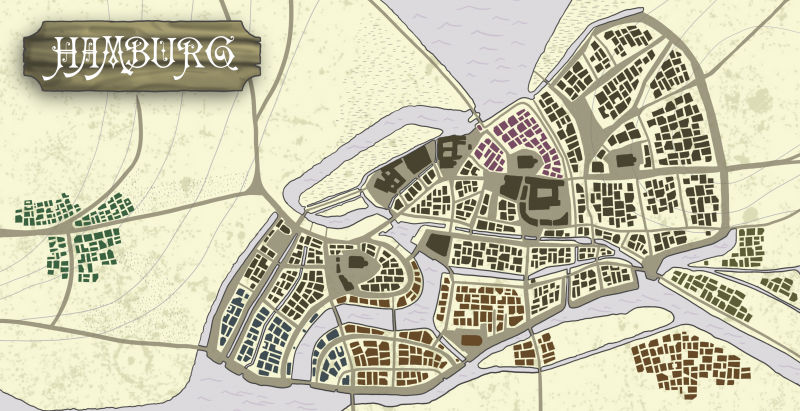
\includegraphics[scale=0.7]{./images/Karte.png}
		\caption{Stadkarte von Hamburg, anno 1350}
    \label{fig:Karte}
	\end{center}
\end{figure}


\subsection{Das Gespräch mit dem Rat}

Also Ihr euch also unterhaltet öffnet sich plötzlich die Holztür und ein junger Ratsdiener bittet euch vor den Rat zu treten.

\red{\textbf{Szene}}: Vor dem Hamburger Rat

\textbf{Raumbeschreibung}: Ihr tretet in einen großen Raum ein, der von einer U-förmigen Tischreihe dominiert werden, an dem 18 Männer in erhöhter Position sitzen. Auch wenn der Raum sonst nur spärlich eingerichtet ist, ist offensichtlich dass sich hier sonst niemand aufhält, der wenig Geld hat. Aus den Wänden sind kunstvoll Löwenköpfe und andere Muster herausgearbeitet. Eine Wand ist von hohen Fenstern gesäumt, die den Raum hell erleuchten.

Im Hintergrund huschen Ratsdiener mit Papieren umher oder gehen anderen Aufgaben nach.

\red{\textbf{Info}: Die 18 Männer setzen sich aus neun Rechtskundigen, sieben Kaufleuten und zwei Vertretern der Kirche zusammen.}

\red{\textbf{Interaktion}}:

Vorsitzender des Rates:
\gqm{\textit{Der Hamburger Rat dankt euch für euer Erscheinen. Bevor wir uns jedoch mit den euch betrauten Aufträgen befassen werden, sagt, was wisst ihr über die Pestilenz?}}

\red{\textbf{Probe auf Gesellschaft/Wissen o.Ä}: Menschen die von der Pestilenz befallen sind leiden unter Schwindelgefühlen und Schüttelfrost. Auch klagen manche über starke Kopfschmerzen und erbrechen sich häufig. Ein hohes Fieber sowie schwarze Pestbeulen an den Lymphknoten treten im Verlaufe der Krankheit auf und sind für den Patienten meist ein sicheres Todeszeichen.}

\red{\textbf{kritischer Erfolg/Probe auf Medizin}: Manche Heiler berichten, dass sie die Pestbeulen aufschneiden und vom darin enthaltenden Eiter reinigen. Wird anschließend das Fieber eines Kranken behandelt konnte mancher Totgeglaubte wieder von der Pest geheilt werden.}

Vorsitzender des Rates:
\gqm{\textit{}}


\section{Kapitel 2 - Im Sitz des Beirats}

%!TEX root = ../main.tex

\red{\textbf{Szene}}:

Nachdem ihr aus dem Rat entlassen wurdet macht ihr euch also auf den Weg zum Sitz des Beirats. In der unmittelbaren Umgebung des Ratshauses spürt man den Aufstieg Hamburgs als Handelsmetropole am deutlichsten. Ihr schlendert durch breite Straßen die von hohen Häusern gesäumt werden. Dienstboten eilen über den Pflasterstein und auch sonst herrscht geschäftiges treiben, als ihr unweit der St. Michaelis Kirche vor eine Kapelle tretet, die euch der Rat als eure Operationszentrale genannt hat

\textbf{Raumbeschreibung}: Als ihr an der kleinen Kapelle ankommt, erkennt ihr, dass es sich dabei um ein durchaus anschauliches Gebäude handelt, dass erst kürzlich einen neuen Anstrich mit weißer Farbe erhalten hat. Im Inneren stehen allerhand Tische und Stühle herum. Außerdem gibt es Schlafmöglichkeiten und so ziemlich alles, was man zum Leben so gebrauchen kann. Selbst ausgewählte Speisen stehen bereits zum Verzehr bereit.

\textbf{Ereignis}: Die Gruppe kann sich erst mal unterhalten. Ihr Gespräch wird allerdings von einem Klopfen unterbrochen ...

\begin{tcolorbox}
  Wurf: Wer oder was unterbricht das Gespräch unserer Gruppe?
  Das Militär (1 bis 33) (gehe zu \ref{militär}) \\
  Der Tod (34 bis 66) (gehe zu \ref{tot}) \\
  Ein Kind (67 bis 99) \ref{kind} \\
  Bei 100: würfle erneut.
\end{tcolorbox}

\section{Der militärische Besuch}
\label{militär}

\red{\textbf{Szene}}:

General zur Brügge steht davor und bittet um Einlass.

Gespräch mit Brügge: Dieser berichtet ihnen in vehementem Ton, dass die ganze Krise ein Werk der Dithmarscher sei. Diese hätten sich jahrelang an Hamburgs Handelsschiffen gütlich getan. Nun, da es einen Vertrag gibt, der das verhindert, versuchen einige von ihnen die Stadt zu schwächen, um davon zu profitieren oder sie gar ganz an sich zu reißen. Die Dithmarscher operieren von ihrem Versteck aus, das sich in einer Hafenkaschemme namens „Beim Gelockten Hund“ befinden soll. Ein gewisser Gorich leite das Ganze. Dort sollten sie mit ihren Recherchen beginnen.

Interaktionen:

Probe auf Menschenkenntnis:

General zur Brügge sagt schon die Wahrheit, aber seine Perspektive könnte durchaus verzerrt beziehungsweise einseitig sein.
Die Charaktere können sich aber sicher sein, dass er nicht lügt, zumindest seiner Auffassung nach nicht.

Ab hier können die Spieler frei entscheiden, wohin sie gehen wollen! Nach Ablauf der Frist von vier Tagen müssen sie beim Hamburger Rat vorsprechen. Bis dahin müssen sie sich auf eine Handlungsempfehlung festgelegt haben!


Option 2 – Der Tod
\red{\textbf{Szene}}:

Ereignis: Während sich die Gruppe noch unterhält, hören die Charaktere plötzlich ein lautes Klopfen an der Tür.

Davor steht der Totensammler Hanno. Er fragt, ob es Tote gäbe, die abzuholen seien, und ob im Haus bereits die Pest wüte.

Gespräch mit Hanno: Im Armenviertel sei es am Schlimmsten. Die Leichen könne er kaum mehr entsorgen. Man müsse kreativ werden.

Gegen Bestechung verrät er, dass er jemandem Leichen verkaufe. Dazu müsse er sie allerdings recht weit fortbringen, nämlich in einen kleinen Ort namens Eeksdurf vor den Toren der Stadt. Dort hinterlege er die leblosen Körper in einem Lagerhaus, wo bereits seine Bezahlung auf ihn warte. Die Absprache habe er dereinst mit einer jungen rothaarigen Frau getroffen.

Sie habe ihn angesprochen, nachdem sie ihn beim Abholen von Leichen im Dorf sah...


Ab hier können die Spieler frei entscheiden, wohin sie gehen wollen! Nach Ablauf der Frist von vier Tagen müssen sie beim Hamburger Rat vorsprechen. Bis dahin müssen sie sich auf eine Handlungsempfehlung festgelegt haben!


Option 3 – Ein Kind
\red{\textbf{Szene}}:

Ereignis: Es klopft plötzlich an der Tür und davor steht ein Kind zusammen mit seiner stark vermummten Mutter.

Gespräch mit der Mutter und dem Kind: Sie kämen aus dem Armenviertel Hammerbrook und seien auf der Suche nach der St. Petri-Kirche. Sie soll ein Zufluchtsort für gesunde und sündenfreie Menschen sein. Niemand werde dort krank! Für sie sei es zu spät, hustet die Frau, aber ihr kleines Kind, das sei noch zu retten. Sie wissen das alles von einem Mann, der im Armenviertel nach den Leuten sehe. Er werde nicht krank, egal was er tue ... Er habe sie losgeschickt. Sie wüssten gern den Weg.

Die Gruppe kann eine Beschreibung von Didrich von Sinnfeld erhalten. Außerdem geben ihnen die beiden auf Nachfrage den Tipp, einmal beim Lumpensammler im Armenviertel vorbeizuschauen.


Ab hier können die Spieler frei entscheiden, wohin sie gehen wollen! Nach Ablauf der Frist von vier Tagen müssen sie beim Hamburger Rat vorsprechen. Bis dahin müssen sie sich auf eine Handlungsempfehlung festgelegt haben!



\end{document}
